\chapter{Appendice Tecnica: Configurazione di un sistema HomeKit}
\section*{Esempio di configurazione YAML per Homebridge}
\begin{verbatim}
{
  "bridge": {
    "name": "Homebridge",
    "username": "CC:22:3D:E3:CE:30",
    "port": 51826,
    "pin": "031-45-154"
  },
  "description": "Configurazione base per accessori BTicino e Netatmo",
  "accessories": [],
  "platforms": [
    {
      "platform": "netatmo",
      "name": "Netatmo Platform",
      "client_id": "TUO_CLIENT_ID",
      "client_secret": "TUO_CLIENT_SECRET",
      "username": "email@example.com",
      "password": "password"
    }
  ]
}
\end{verbatim}

\section*{Schermata di esempio}
\begin{figure}[h!]
    \centering
    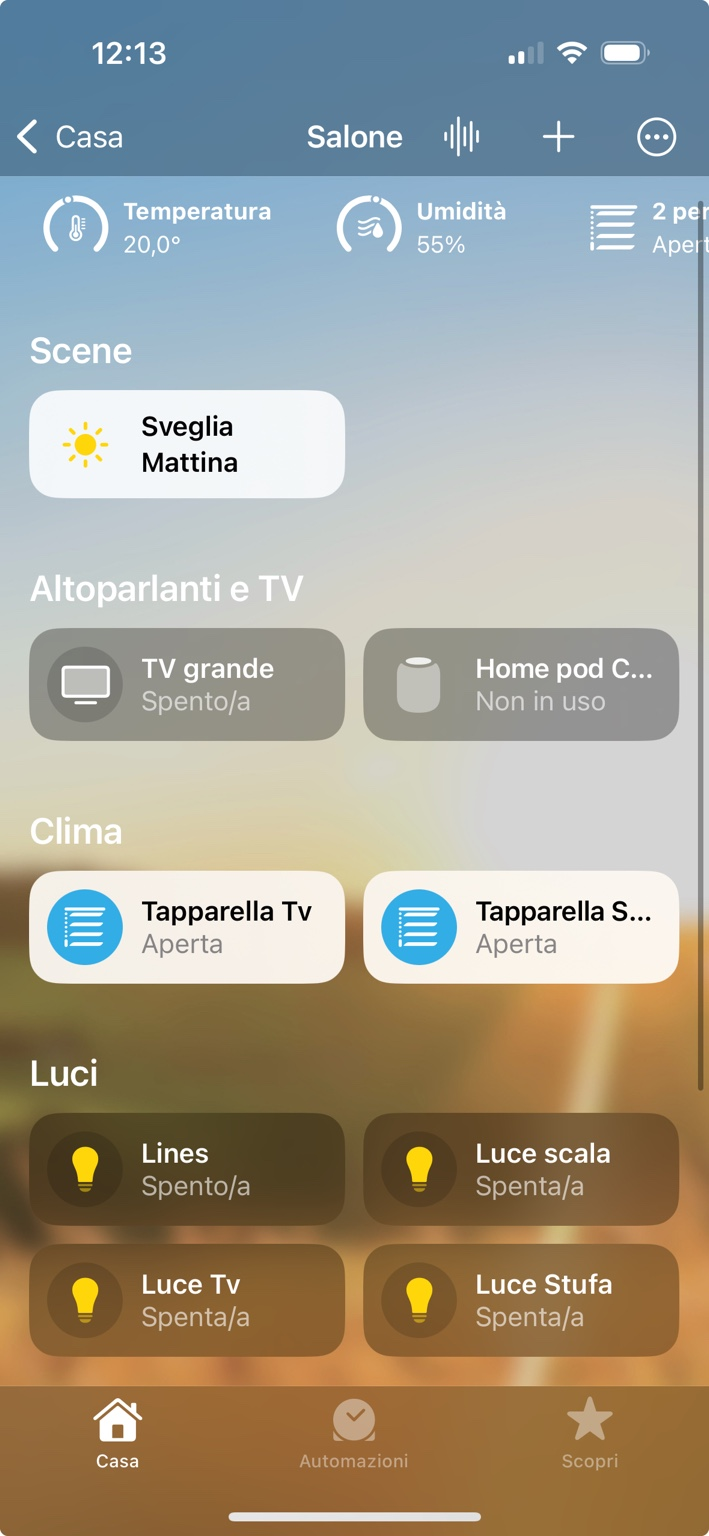
\includegraphics[scale=0.13]{immagini/esempio-homekit.jpeg}
    \caption{Interfaccia Apple Home con dispositivi configurati}
    \label{fig:homekit-interface}
\end{figure}

